\documentclass{article}

\usepackage{graphicx}
\usepackage[brazil]{babel}
\usepackage{subcaption}
\usepackage{amsmath}
\usepackage{float}
\usepackage{listings}
\usepackage{hyperref}
\usepackage{xcolor}
\usepackage{tikz}
\usepackage{pgfplots}
% \usepackage{subfig}
\pgfplotsset{compat=1.18}
\lstset{
    language=C,
    basicstyle=\ttfamily\footnotesize,
    keywordstyle=\color{blue},
    stringstyle=\color{red},
    commentstyle=\color{green},
    breaklines=true,
    numbers=left,
    numberstyle=\tiny\color{gray},
    stepnumber=1,
    numbersep=5pt,
    showspaces=false,
    showstringspaces=false,
    tabsize=2
}

\newcommand{\plotHistogram}[1]{
    \pgfplotstableread{../dat/#1_mean.dat}\loadedtable
    \pgfplotstablegetelem{0}{[index]0}\of\loadedtable
    \edef\meanvalue{\pgfplotsretval}
    \pgfplotstableread{../dat/#1_count.dat}\loadedtable
    \pgfplotstablegetelem{0}{[index]0}\of\loadedtable
    \edef\countvalue{\pgfplotsretval}
            \begin{tikzpicture}
                \begin{axis}[
                    xlabel=Número de elementos,
                    ylabel=Contagem,
                    bar width=0.01cm,
                    legend pos=outer north east,
                    width=0.9\textwidth,
                    height=0.25\textwidth,
                ]
                \addplot[ybar, fill=black!50, draw=black!50] table {../dat/#1.dat};
                \draw[gray, dashed] (axis cs:\meanvalue, 0) -- (axis cs:\meanvalue, \countvalue);
                \addlegendentry{Média};
                \end{axis}
            \end{tikzpicture}
            }

\newcommand{\plotHistogramW}[1]{
            \begin{tikzpicture}
                \begin{axis}[
                    xlabel=Número de elementos,
                    ylabel=Contagem,
                    bar width=0.01cm,
                    legend pos=outer north east,
                    width=0.9\textwidth,
                    height=0.25\textwidth,
                ]
                \addplot[ybar, fill=black!50, draw=black!50] table {../dat/#1.dat};
                %\draw[gray, dashed] (axis cs:\meanvalue, 0) -- (axis cs:\meanvalue, \countvalue);
                %\addlegendentry{Média};
                \end{axis}
            \end{tikzpicture}
            }
\newcommand{\plotHistogramLog}[1]{
            \pgfplotstableread{../dat/#1_mean.dat}\meanvalue
            \pgfplotstableread{../dat/#1_count.dat}\countvalue
            \begin{tikzpicture}
                \begin{semilogyaxis}[
                    xlabel=Número de elementos,
                    ylabel=Contagem,
                    bar width=0.01cm,
                    legend pos=outer north east,
                    width=0.9\textwidth,
                    height=0.4\textwidth,
                ]
                \addplot[ybar, fill=black!50, draw=black!50] table {../dat/#1.dat};
                \draw[gray, dashed] (\meanvalue, 0) -- (\meanvalue, \countvalue);
                \addlegendentry{Média};
                \end{semilogyaxis}
            \end{tikzpicture}
            }
\newcommand{\plotComparison}[2]{
    \begin{figure}[H]
        \centering
        \begin{subfigure}[b]{0.3\textwidth}
            \includegraphics[width=\textwidth]{../imags/#1.png}
            \caption{Imagem Original #2}
            \label{fig:original_#1}
        \end{subfigure}
        \hfill
        \begin{subfigure}[b]{0.3\textwidth}
            \includegraphics[width=\textwidth, angle=180]{../imags/#1_laplacian.png}
            \caption{Filtro Laplaciano #2}
            \label{fig:laplacian_#1}
        \end{subfigure}
        \hfill
        \begin{subfigure}[b]{0.3\textwidth}
            \includegraphics[width=\textwidth, angle=180]{../imags/#1_high-boost.png}
            \caption{High-Boost #2}
            \label{fig:highboost_#1}
        \end{subfigure}
        \caption{Comparação entre a imagem original, a imagem com filtro Laplaciano e a imagem com realce de High-Boost #2.}
        \label{fig:comparacao_#1}
    \end{figure}
}
\newcommand{\plotHistogramWs}[2]{
    \begin{figure}[H]
        \centering
        \plotHistogramW{#1}
        \caption{Histograma Imagem original #2.}
        \label{fig:hist1_#1}
    \end{figure}

    \begin{figure}[H]
        \centering
        \plotHistogramW{#1_laplacian}
        \caption{Histograma filtro Laplaciano #2.}
        \label{fig:hist2_#1}
    \end{figure}

    \begin{figure}[H]
        \centering
        \plotHistogramW{#1_high-boost}
        \caption{Histograma realce de High-Boost #2.}
        \label{fig:hist3_#1}
    \end{figure}
}
\newcommand{\plotHistograms}[2]{
    \begin{figure}[H]
        \centering
        \plotHistogram{#1}
        \caption{Histograma Imagem original #2.}
        \label{fig:hist1_#1}
    \end{figure}

    \begin{figure}[H]
        \centering
        \plotHistogram{#1_laplacian}
        \caption{Histograma filtro Laplaciano #2.}
        \label{fig:hist2_#1}
    \end{figure}

    \begin{figure}[H]
        \centering
        \plotHistogram{#1_high-boost}
        \caption{Histograma realce de High-Boost #2.}
        \label{fig:hist3_#1}
    \end{figure}
}
            
\author{Davi de Lima Cruz\\  PROJETO 02-2024.2: Grupo 1}
\title{Relatório: Realce de imagens usando o Laplaciano e Filtragem Espacial}
\date{11 de dezembro de 2024}

\begin{document}
\maketitle

\vfill
\section*{Resumo}
Este relatório apresenta a aplicação de técnicas de realce de imagem utilizando o filtro Laplaciano e o realce de High-Boost. A biblioteca libtiff foi utilizada para leitura e escrita de imagens no formato TIFF. Os resultados foram analisados por meio de comparações visuais e histogramas, demonstrando a eficácia das técnicas aplicadas.
\newpage
\section{Discussão Técnica}
\subsection{Biblioteca libtiff e Histograma}
Para a leitura e escrita de imagens, foi usada a biblioteca \href{http://www.simplesystems.org/libtiff/}{libtiff} que pode ser instalada no linux com o comando \texttt{sudo apt-get install libtiff-dev}. 
Para compilar o programa, foi utilizado o seguinte comando:
\begin{lstlisting}
    gcc -o app main.c -ltiff
\end{lstlisting}
O programa aceita dois argumentos: 
\begin{lstlisting}
    ./app <command> <filename> [<k>]
\end{lstlisting}
onde:
\begin{itemize}
    \item \texttt{<command>} pode ser \texttt{hist}, \texttt{laplacian} ou \texttt{high-boost}.
    \item \texttt{<filename>} é o nome do arquivo TIFF (sem a extensão .tif).
    \item \texttt{<k>} é um parâmetro usado nos comandos \texttt{laplacian} e \texttt{high-boost} para definir a constante $k$.
\end{itemize}

\subsection{Filtro Laplaciano}
O filtro Laplaciano é um operador de detecção de bordas que realça as regiões de alta frequência na imagem. Ele é útil para destacar as bordas e os detalhes finos na imagem. O programa aplica o filtro Laplaciano em uma uma mascara 3x3 e, em seguida, combina a imagem original com a imagem filtrada usando uma constante ajustável.
Para essa aplicação, foi utilizado o seguinte kernel:
\[
\begin{bmatrix}
0 & -1 & 0 \\
-1 & 4 & -1 \\
0 & -1 & 0
\end{bmatrix}
\]
e a constante foi definida como -1.

\subsection{Realce de High-Boost}
O realce de high-boost é uma técnica de realce de imagem que realça as regiões de alta frequência na imagem. Ele é útil para realçar os detalhes finos e melhorar a nitidez da imagem. O programa aplica o realce de high-boost em uma imagem usando a seguinte fórmula:
\[
f_{\text{realcada}}(x,y) = f_{\text{original}}(x,y) + k \times (f_{\text{original}}(x,y) - f_{\text{suavizada}}(x,y))
\]
onde $k$ é um parâmetro ajustável que controla a intensidade do realce. Para essa aplicação, a constante foi definida como 4,5.
Para a imagem suavizada, foi utilizado um filtro gaussiano com kernel 3x3 e desvio padrão 5.
\section{Discussão dos Resultados}
Os histogramas das imagens 3-33 e 3-38 do livro não são muito didáticos para explicar as diferenças entre as imagens originais e as imagens com filtro Laplaciano e realce de High-Boost. Por isso, foi utiliza a imagem da praia para ilustrar as diferenças entre as imagens originais e as imagens com filtro Laplaciano e realce de High-Boost.
%%% praia
\begin{figure}[H]
    \centering
    \begin{subfigure}[b]{0.3\textwidth}
        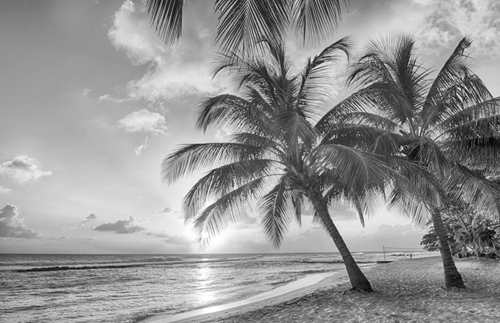
\includegraphics[width=\textwidth]{../imags/praia.png}
        \caption{Imagem Original}
        \label{fig:original_praia}
    \end{subfigure}
    \hfill
    \begin{subfigure}[b]{0.3\textwidth}
        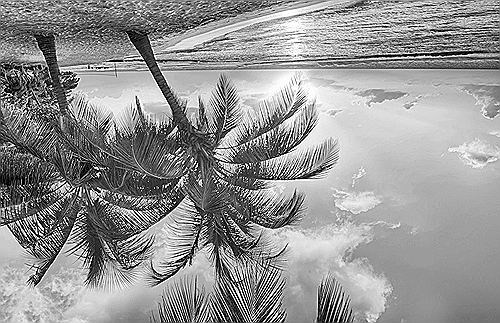
\includegraphics[width=\textwidth, angle=180]{../imags/praia_laplacian.png}
        \caption{Filtro Laplaciano}
        \label{fig:laplacian_praia}
    \end{subfigure}
    \hfill
    \begin{subfigure}[b]{0.3\textwidth}
        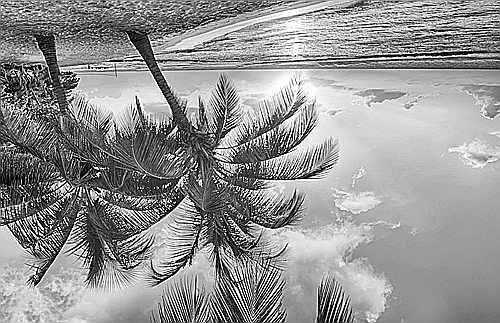
\includegraphics[width=\textwidth, angle=180]{../imags/praia_high-boost.png}
        \caption{Realce de High-Boost}
        \label{fig:highboost_praia}
    \end{subfigure}
    \caption{Comparação entre a imagem original, a imagem com filtro Laplaciano e a imagem com realce de High-Boost.}
    \label{fig:comparacao_praia}
\end{figure}

\begin{figure}[H]
    \centering
    \plotHistogram{praia}
    \caption{Histograma Imagem original.}
    \label{fig:hist1_praia}
\end{figure}

\begin{figure}[H]
    \centering
    \plotHistogram{praia_laplacian}
    \caption{Histograma filtro Laplaciano.}
    \label{fig:hist2_praia}
\end{figure}

\begin{figure}[H]
    \centering
    \plotHistogram{praia_high-boost}
    \caption{Histograma realce de High-Boost.}
    \label{fig:hist3_praia}
\end{figure}
Os resultados apresentados nas Figuras \ref{fig:comparacao_praia}, \ref{fig:hist1_praia}, \ref{fig:hist2_praia} e \ref{fig:hist3_praia} mostram a comparação entre a imagem original, a imagem com filtro Laplaciano e a imagem com realce de High-Boost, bem como seus respectivos histogramas.

Na Figura \ref{fig:comparacao_praia}, podemos observar que o filtro Laplaciano realça as bordas da imagem, destacando os detalhes finos. Já o realce de High-Boost aumenta a nitidez da imagem, tornando os detalhes mais visíveis.

Os histogramas das Figuras \ref{fig:hist1_praia}, \ref{fig:hist2_praia} e \ref{fig:hist3_praia} mostram a distribuição dos níveis de cinza nas imagens. O histograma da imagem original (Figura \ref{fig:hist1_praia}) apresenta uma distribuição mais uniforme, enquanto o histograma da imagem com filtro Laplaciano (Figura \ref{fig:hist2_praia}) mostra um aumento na frequência dos níveis de cinza correspondentes às bordas. O histograma da imagem com realce de High-Boost (Figura \ref{fig:hist3_praia}) apresenta picos mais acentuados, indicando um aumento no contraste da imagem.

\plotComparison{338}{3-38}
As imagens 3-33 e 3-38 têm histogramas semelhantes, com uma distribuição nenhum pouco uniforme. Tornando a analise visual mais difícil. No entanto, segue os histogramas das imagens 3-33 e 3-38.
\plotHistograms{338}{3-38}
\plotComparison{333}{3-33}
\plotHistograms{333}{3-33}
A outra foto utilizada foi a da mulher, que apresenta um histograma mais uniforme, facilitando a análise visual. Tendo a mesma explicação do histograma anterior, onde o filtro Laplaciano realça as bordas da imagem, destacando os detalhes finos. Já o realce de High-Boost aumenta a nitidez da imagem, tornando os detalhes mais visíveis.
Basicamente, o histograma vai mais para os extremos, mostrando que a imagem foi realçada.
\plotComparison{mulher}{Mulher}
\plotHistogramWs{mulher}{Mulher}

    \section{Código Fonte em C}
\lstinputlisting[language=C, caption={Código fonte do programa em C.}]{../src/main.c}


\end{document}
